\documentclass[10pt,conference,draftclsnofoot,onecolumn]{IEEEtran}
\usepackage{listings}
\usepackage[dvipsnames]{xcolor}
\usepackage{graphicx}
\usepackage{color}
\usepackage{anysize}
\usepackage{hyperref}
\usepackage[backend=bibtex]{biblatex}
\usepackage{amsmath}
\marginsize{2cm}{2cm}{2cm}{2cm}
\addbibresource{bib.bib}

\lstdefinelanguage
   [x86Extended]{Assembler}     % add an "x86Extended dialect of Assembler
   [x86masm]{Assembler}         % based on the "x86masm" dialect
   % Define new keywords
   {morekeywords={rdrand, cpuid}}

\lstdefinestyle{customc}{
  belowcaptionskip=1\baselineskip,
  breaklines=true,
  frame=L,
  xleftmargin=\parindent,
  language=C,
  showstringspaces=false,
  basicstyle=\footnotesize\ttfamily,
  keywordstyle=\bfseries\color{OliveGreen},
  commentstyle=\itshape\color{Fuchsia},
  identifierstyle=\color{black},
  stringstyle=\color{Bittersweet},
}

\lstdefinestyle{customasm}{
  belowcaptionskip=1\baselineskip,
  frame=L,
  xleftmargin=\parindent,
  language=[x86masm]Assembler,
  basicstyle=\footnotesize\ttfamily,
  commentstyle=\itshape\color{Fuchsia},
}

\lstset{escapechar=@,style=customc}


\begin{document}

\begin{titlepage}
    \centering
    {\scshape\LARGE Oregon State University \par}
    \vspace{1cm}
    \vspace{1cm}
    {\scshape\Large Operating System Feature Comparison \par}
    \vspace{1.5cm}
    {\huge\bfseries I/O \& Provided Functionality \par}
    \vspace{2cm}
    {\Large\itshape Ian Kronquist \par}
    \vfill
    \par
    {\scshape\Large CS 444 Operating Systems II \par}
    {\scshape\Large Spring 2016\par}

    \vspace{3cm}
    Professor~Kevin \textsc{McGrath}
    \vfill

% Bottom of the page
    {\large \today\par}
\end{titlepage}


\author{\IEEEauthorblockN{Ian Kronquist}
\IEEEauthorblockA{School of Electrical and\\Computer Science\\
Oregon State University\\
Corvallis, Oregon\\
kronquii@oregonstate.edu}}

\bigskip

\section{Introduction}
For this assignment we will examine processes, threads, and scheduling in four different kernels: Linux, Windows NT, FreeBSD, and XNU Darwin.
Linux is an open source GPL licensed monolithic kernel from the UNIX tradition. Development started in 1991 by Linus Torvalds. It was originally intended as an educational project to learn more about operating systems and to port Minix, an older educational kernel, and to port it to the 80386 computer he owned at the time\cite{1_love_2010}.

The Windows NT 3.1 kernel was originally released in 1993. Windows is uniquely intertwined with its windowing system and display driver code, and has a novel idea of subsystems. Subsystems can provide different APIs such as MS-DOS, Windows 16, Windows 32, or even a POSIX compliant subsystem\cite{2_russinovich_solomon_ionescu_2012}.

The FreeBSD operating System is a fork of the original BSD operating system. The early 4.3 BSD operating system was produced in 1983\cite{3_mckusick_neville-neil_watson_2015}. FreeBSD is, shockingly enough, BSD licensed, and is the more permissively licensed of these three operating systems.

\section{I/O Scheduling}
I/O is the slowest thing computers do. Operating systems can try to speed up I/O by scheduling I/O requests to disks to try to take advantage of the capabilities of the hardware.


\subsection{Linux I/O Schedulers}
Linux uses an innovative pluggable system to schedule I/O requests to devices like hard disks and solid state drives. Linus wrote the original scheduler, sometimes called the Linus Elevator, but as Linux usage spread to a variety of systems including desktop, server, supercomputers, and embedded, it was discovered that the algorithm which Linus developed wasn't a good fit for all devices and all use cases. As a result, work was begun on a system which allows drivers or users to select the proper I/O scheduler at runtime\cite{1_love_2010}. Each scheduler defines a series of I/O operations in a structure called \texttt{elevator\_ops}. This structure defines the scheduler's name, what functionality the scheduler implements, such as whether or not it does merging, and provides a series of function pointers which allow the kernel to pass requests to the scheduler for processing\cite{5_torvalds_2016}.

\lstset{language=C,caption={Linux Kernel \texttt{elevator\_ops} Data Structure},label=process}
\begin{lstlisting}
struct elevator_ops
{
	elevator_merge_fn *elevator_merge_fn;
	elevator_merged_fn *elevator_merged_fn;
	elevator_merge_req_fn *elevator_merge_req_fn;
	elevator_allow_merge_fn *elevator_allow_merge_fn;
	elevator_bio_merged_fn *elevator_bio_merged_fn;

	elevator_dispatch_fn *elevator_dispatch_fn;
	elevator_add_req_fn *elevator_add_req_fn;
	elevator_activate_req_fn *elevator_activate_req_fn;
	elevator_deactivate_req_fn *elevator_deactivate_req_fn;

	elevator_completed_req_fn *elevator_completed_req_fn;

	elevator_request_list_fn *elevator_former_req_fn;
	elevator_request_list_fn *elevator_latter_req_fn;

	elevator_init_icq_fn *elevator_init_icq_fn;	/* see iocontext.h */
	elevator_exit_icq_fn *elevator_exit_icq_fn;	/* ditto */

	elevator_set_req_fn *elevator_set_req_fn;
	elevator_put_req_fn *elevator_put_req_fn;

	elevator_may_queue_fn *elevator_may_queue_fn;

	elevator_init_fn *elevator_init_fn;
	elevator_exit_fn *elevator_exit_fn;
};
\end{lstlisting}

Each scheduler can register itself by calling \texttt{elevator\_register} and
unregister itself by calling \texttt{elevator\_unregister}. Elevators set can choose whether they want to implement all of the features which kernel supports. One such feature which isn't always implemented is merging. Merging is the process of taking two requests at adjacent sectors and combining them into one request to reduce the number of requests issued. Merging is useful for devices, like hard disks, where servicing requests is expensive. However, other storage drivers like solid state drives have built-in controller schedulers, so there is no need to perform much scheduling or merging when the hardware will do it faster anyway\cite{1_love_2010}.

The Linux 3.14 kernel comes with three schedulers by default: the Completely Fair Queue, or CFQ, scheduler, the Deadline scheduler, and the Noop scheduler. The CFQ I/O scheduler is the default scheduler and is best adapted to a wide variety of workloads. Like the CFQ process scheduler, it tries to give all processes requesting access to the disk a fair share of the disks resources so a single process' I/O is not unfairly delayed. This is especially important on desktop systems which have a high rate of user interactivity. However, for some I/O heavy server tasks another solution is called for. The Deadline scheduler tries to reduce the possibility of resource starvation at the expense of throughput. Certain devices like solid state drives have built-in hardware controllers which perform their own scheduling, and so providing an additional layer of scheduling will only decrease latency. These devices are best served by the Noop scheduler, which just sticks all requests into a queue and pops them off when they're asked for\cite{1_love_2010}.

Interestingly enough, Qualcomm attempted to merge a scheduler optimized for mobile devices called the ROW or ``Read Over Write'' scheduler. This scheduler attempts to prioritize reads for a faster user experience\cite{lkml-row-patch}. The Linux kernel developers rather dispassionately rejected the patch after calling for more testing and not reading the documentation included in the patch\cite{lkml-row-patch-rejection}. The ROW scheduler is included in the Android 6 kernel.

\subsection{Windows I/O}
Windows has two I/O prioritization strategies called the Hierarchical Strategy and the Idle Strategy which are used for different drivers. Certain I/O requests can skip this scheduling layer altogether and hand off information directly to the driver via a mechanism called Fast I/O. The ATA and USB port drivers implement the Hierarchy Strategy, and the SCSI and storage port drivers do not.

The Hierarchical strategy prioritizes certain I/O operations so that tasks like indexing and scanning for viruses don't affect other important operations. There are five levels of I/O priority: Critical, High, Normal, Low, Very Low. The memory manager has Critical priority, and normal user tasks have Normal priority. Tasks like virus scanning and disk defragmentation have very low priority. Requests are placed on different queues, and all Critical requests are processed before Normal requests and so on. Additionally, all requests made by kernel mode code and requests having to do with paging have at least Normal priority.

The Idle Strategy places requests on a simple queue. The scheduler uses a timer to monitor the Idle queue and make sure that at least one request is pulled off of the queue every half a second. Additionally, the scheduler waits for 50ms after the last Hierarchical request to issue the next request so that Idle requests don't interrupt high priority requests and cause unnecessary disk thrashing\cite{2_russinovich_solomon_ionescu_2012}.

\subsection{FreeBSD I/O}
FreeBSD does not have a pluggable I/O scheduler system like Linux. Instead, it uses a single dedicated scheduler called CAM for all workloads. NetFlix rewrote parts of the CAM scheduler to optimize it for their SSD workload, and it is still under active development. Certain disk drivers bypass the CAM layer altogether and implement their own scheduling algorithms. The new NetFlix scheduling algorithm prioritizes reads over writes like Linux's CFQ and ROW schedulers, since reading is faster than writing for both SSDs and HDs. The NetFlix scheduler also has two ``limiters'' which can be enabled to affect I/O performance. It has a fairness bias limiter to ensure that different types of requests, such as reads, writes, and deletes, get fair usage of devices, and it has a queue depth limit which prevents the queues from growing too long. It also has a bandwidth limiter and an I/O operations per second limiter which can be tuned for different disks.

\begin{figure}[h]
    \centering
    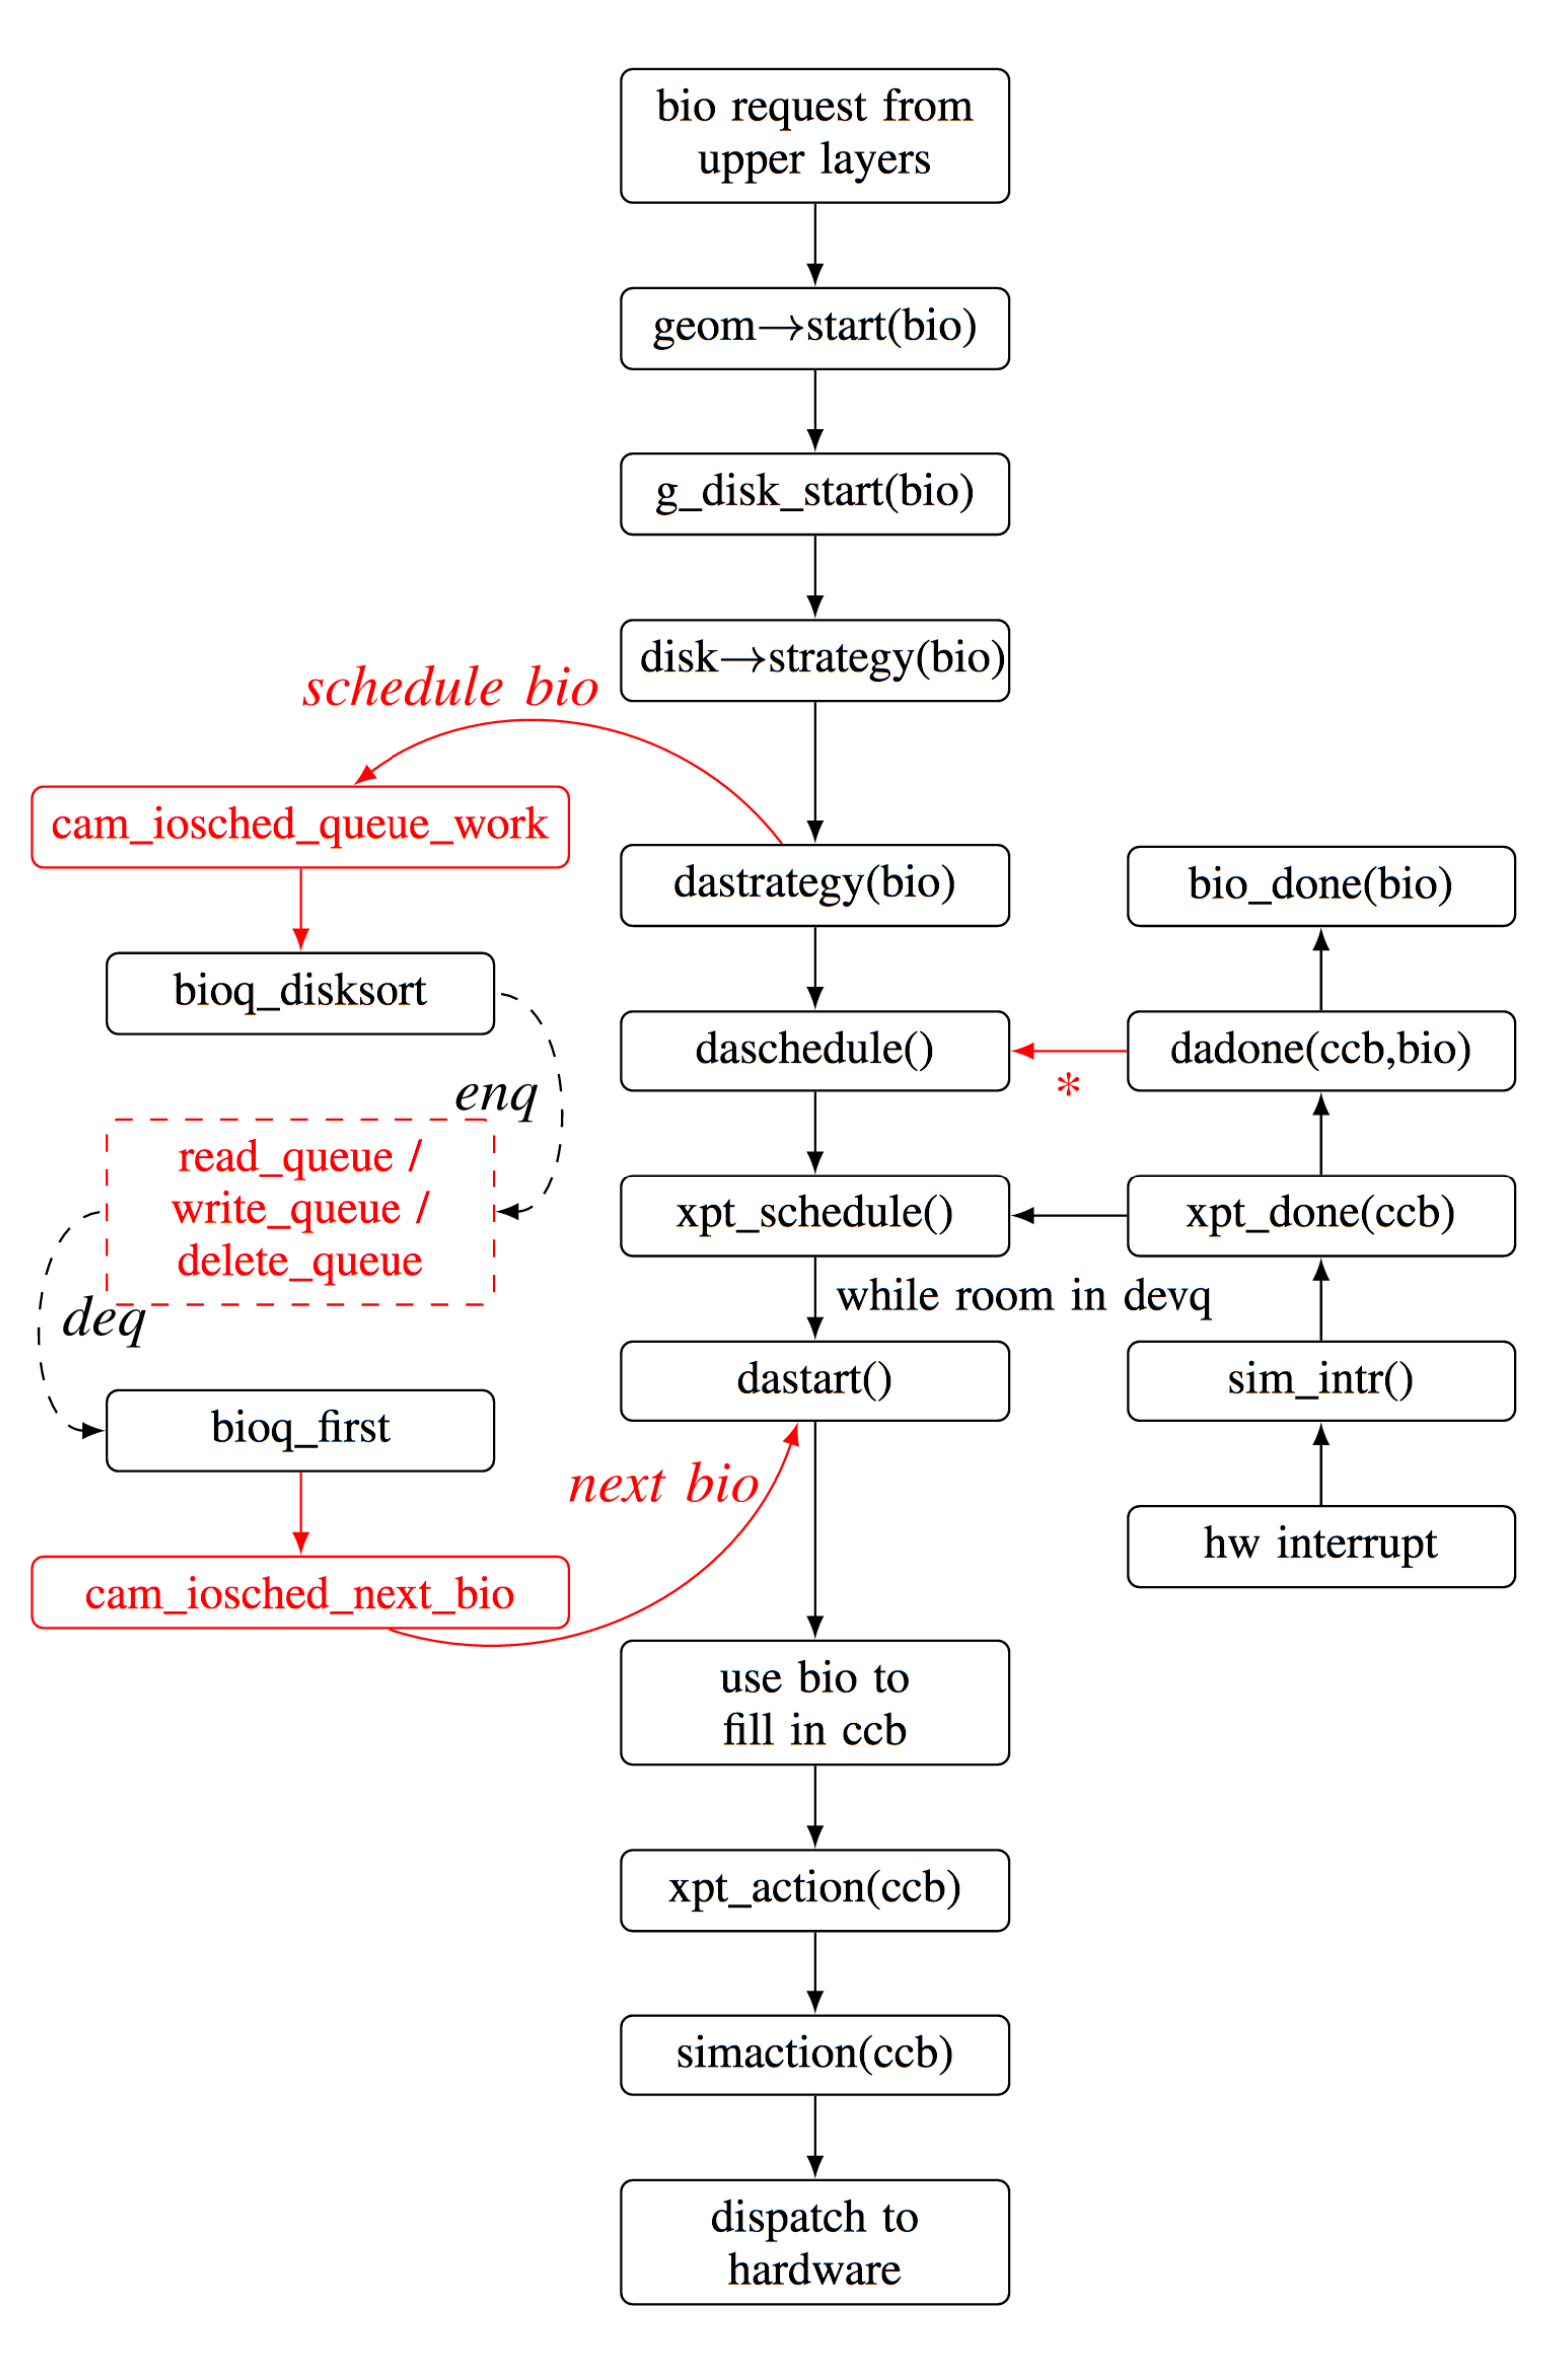
\includegraphics[width=0.4\textwidth]{netflix-ioshed.eps}
    \caption{FreeBSD I/O Stack With NetFlix Scheduler}
\end{figure}

The NetFlix scheduler cannot prioritize I/O from certain users or processors or implement any quotas. Unfortunately, it cannot propagate feedback about full I/O pipelines to the upper layers of the system.
Currently the NetFlix engineers are working on tuning a Phased Locked Loop like steering feedback loop to observe the disk's read and write performance and inhibit the number of reads or writes issued. This fascinating little algorithm can be found in the appendix. Overall, Linux's scheduler system is far more advanced and flexible than FreeBSD's implementation.

\section{Included Functionality: File Systems}
Some of the most interesting sort of OS specific information are the supported file systems. Modern operating systems can support a variety of different file systems, however they all have one which is most commonly used. In this section we'll examine Linux's EXT4, FreeBSD's ZFS, and Windows' NTFS.
\subsection{EXT4}
EXT4 is, unsurprisingly, the fourth generation of the EXT family of file systems. It is the most widely used file system on Linux systems. It is a case sensitive, journaled file system. EXT4 can store much more data than its EXT3 predecessor. It currently supports files and file systems up to 16 Terabytes. Existing EXT3 file systems are forward compatible with EXT4, and can be upgraded incredibly easily by just changing a few settings. Like NTFS and ZFS EXT4 has online defragmentation so that inefficiently used disk space can be reused while the OS is running. Similarly to NTFS EXT4 has quotas for users and groups\cite{ext4-perf}.

\subsection{ZFS}
ZFS is one of the most interesting modern file systems. Like EXT4 and any other modern file system it is case sensitive and journaled. It was originally developed by Sun, and later Oracle, for their Solaris operating system. ZFS is a log structured file system which endeavors not to overwrite existing data. This allows disk snapshots to be created quickly with littler performance hit, which leads to fast backups. Additionally, the ZFS file system is never inconsistent, so even if the computer crashes in the middle of a write operation it is not compromised. Additionally, multiple disks can be pooled together and treated as a single volume. ZFS runs extremely well on systems with tons of memory, but it isn't well suited to embedded systems or 32-bit systems with less than 8 gigabytes of memory\cite{3_mckusick_neville-neil_watson_2015}.

\subsection{NTFS}
Windows' NTFS is, surprisingly, case insensitive. Git can sometimes struggle checking out files on case insensitive file systems if two files in a repository only differ by case. This can make tasks like checking out the Linux source tree surprisingly obnoxious. According to an anonymous Microsoft employee, \textit{``the NTFS code is a purple opium-fueled Victorian horror novel that uses global recursive locks and SEH for flow control''}\cite{windows-kernel-rant}. Unlike older file systems, NTFS supports Unicode file names, hard links, soft links, encryption, and defragmentation. NTFS files can have multiple streams, which are long strings of bytes. Each file by default has a single unnamed stream, but additional named streams can be accessed by appending a colon to the file name, followed by the name of the stream. Different streams might be used by backup utilities, or the Attachment Execution Service which warns users that they are about to execute a file which cam from an untrusted zone like the internet. It also allows per-user volume quotas. Additionally, NTFS has dynamic partitioning allowing partitions to be grown or shrunk at runtime\cite{2_russinovich_solomon_ionescu_2012}.

\lstset{language=,caption={Output of \texttt{git status} on a Case Insensitive File System},label=process}
\begin{lstlisting}
$ git status
On branch master
Your branch is up-to-date with 'origin/master'.
Changes not staged for commit:
  (use "git add <file>..." to update what will be committed)
  (use "git checkout -- <file>..." to discard changes in working directory)

    modified:   include/uapi/linux/netfilter/xt_CONNMARK.h
    modified:   include/uapi/linux/netfilter/xt_DSCP.h
    modified:   include/uapi/linux/netfilter/xt_MARK.h
    modified:   include/uapi/linux/netfilter/xt_RATEEST.h
    modified:   include/uapi/linux/netfilter/xt_TCPMSS.h
    modified:   include/uapi/linux/netfilter_ipv4/ipt_ECN.h
    modified:   include/uapi/linux/netfilter_ipv4/ipt_TTL.h
    modified:   include/uapi/linux/netfilter_ipv6/ip6t_HL.h
    modified:   net/netfilter/xt_DSCP.c
    modified:   net/netfilter/xt_HL.c
    modified:   net/netfilter/xt_RATEEST.c
    modified:   net/netfilter/xt_TCPMSS.c

no changes added to commit (use "git add" and/or "git commit -a")
\end{lstlisting}

\section{Conclusion}
Ensuring fast and fair access to I/O resources like hard disks and solid state drives is one of an operating systems most important tasks. On top of these primitives complex file systems can be built which can help ensure that data is secure from other users and safe in the event of unexpected power failure.

\clearpage
\printbibliography

\clearpage

\begin{appendices}
\section{FreeBSD Steering Engine}

\lstset{language=C,caption={FreeBSD Steering Engine},label=process}
\begin{lstlisting}
static void
cam_iosched_cl_maybe_steer(struct control_loop *clp)
{
	struct cam_iosched_softc *isc;
	sbintime_t now, lat;
	int old;

	isc = clp->softc;
	now = isc->last_time;
	if (now < clp->next_steer)
		return;

	clp->next_steer = now + clp->steer_interval;
	switch (clp->type) {
	case set_max:
		if (isc->write_stats.current != isc->write_stats.max)
			printf("Steering write from %d kBps to %d kBps\n",
			    isc->write_stats.current, isc->write_stats.max);
		isc->read_stats.current = isc->read_stats.max;
		isc->write_stats.current = isc->write_stats.max;
		isc->trim_stats.current = isc->trim_stats.max;
		break;
	case read_latency:
		old = isc->write_stats.current;
		lat = isc->read_stats.ema;
		/*
		 * Simple PLL-like engine. Since we're steering to a range for
		 * the SP (set point) that makes things a little more
		 * complicated. In addition, we're not directly controlling our
		 * PV (process variable), the read latency, but instead are
		 * manipulating the write bandwidth limit for our MV
		 * (manipulation variable), analysis of this code gets a bit
		 * messy. Also, the MV is a very noisy control surface for read
		 * latency since it is affected by many hidden processes inside
		 * the device which change how responsive read latency will be
		 * in reaction to changes in write bandwidth. Unlike the classic
		 * boiler control PLL. this may result in over-steering while
		 * the SSD takes its time to react to the new, lower load. This
		 * is why we use a relatively low alpha of between .1 and .25 to
		 * compensate for this effect. At .1, it takes ~22 steering
		 * intervals to back off by a factor of 10. At .2 it only takes
		 * ~10. At .25 it only takes ~8. However some preliminary data
		 * from the SSD drives suggests a reasponse time in 10's of
		 * seconds before latency drops regardless of the new write
		 * rate. Careful observation will be reqiured to tune this
		 * effectively.
		 *
		 * Also, when there's no read traffic, we jack up the write
		 * limit too regardless of the last read latency.  10 is
		 * somewhat arbitrary.
		 */
		if (lat < clp->lolat || isc->read_stats.total - clp->last_count < 10)
			isc->write_stats.current = isc->write_stats.current *
			    (100 + clp->alpha) / 100;	/* Scale up */
		else if (lat > clp->hilat)
			isc->write_stats.current = isc->write_stats.current *
			    (100 - clp->alpha) / 100;	/* Scale down */
		clp->last_count = isc->read_stats.total;

		/*
		 * Even if we don't steer, per se, enforce the min/max limits as
		 * those may have changed.
		 */
		if (isc->write_stats.current < isc->write_stats.min)
			isc->write_stats.current = isc->write_stats.min;
		if (isc->write_stats.current > isc->write_stats.max)
			isc->write_stats.current = isc->write_stats.max;
		if (old != isc->write_stats.current && 	iosched_debug)
			printf("Steering write from %d kBps to %d kBps due to latency of %jdms\n",
			    old, isc->write_stats.current,
			    (uintmax_t)((uint64_t)1000000 * (uint32_t)lat) >> 32);
		break;
	case cl_max:
		break;
	}
}
\end{lstlisting}
\end{appendices}
\end{document}
\bibliography{bib.bib}
\bibliographystyle{IEEEtran}
